\documentclass[10pt,xcolor={usenames,dvipsnames}]{beamer} %[handout,red]
\usepackage{amsmath}
\usepackage{graphicx,multimedia,hyperref,subfig,tikz}
\usepackage{makecell}
\usepackage[utf8]{inputenc}
\usepackage[czech]{babel}
\usepackage{lmodern}
\usepackage{mathtools}
\usepackage[absolute,overlay]{textpos}
%\usepackage{minted}

\usetikzlibrary{calc}

%%%%%%%%%%%%%%%%%%%%%%%%%%%%%%%%%%%%%%%%%%%%%%%%%%%%%%%%%%%%%%%%%%%%%%%%%%%%%%%%
% SYMBOLS
% \def\div{\operatorname{div}}
% \def\Lapl{\Delta}
% \def\grad{\nabla}
% \def\supp{{\rm supp}}
% \def\dist{{\rm dist}}

% \def\Tr{{\rm Tr}}
% \def\sgn{{\rm sgn}}
% \def\to{\rightarrow}
% \def\weakto{\rightharpoonup}
% \def\imbed{\hookrightarrow}
% \def\cimbed{\subset\subset}
% \def\range{{\mathcal R}}
% \def\argdot{{\hspace{0.18em}\cdot\hspace{0.18em}}}
% \def\Distr{{\mathcal D}}
% \def\convol{\star}
% \def\impl{\Rightarrow}
% \DeclareMathOperator*{\esslim}{esslim}
% \DeclareMathOperator*{\esssup}{ess\,sup}
% \DeclareMathOperator{\ess}{ess}
% \DeclareMathOperator{\osc}{osc}
% \DeclareMathOperator{\curl}{curl}

% ****************************************** GENERAL MATH NOTATION
% \def\Real{{\rm\bf R}}
% \def\d{\,{\rm d}}               % differential



% ******************************************* DOCUMENT NOTATIONS
% document specific
\newcommand{\blk}[2]{\begin{exampleblock}{#1}#2\end{exampleblock}}
\newcommand\diag[4]{%
  \multicolumn{1}{|p{#2}|}{\hskip-\tabcolsep
  $\vcenter{\begin{tikzpicture}[baseline=0,anchor=south west,inner sep=#1]
  \path[use as bounding box] (0,0) rectangle (#2+2\tabcolsep,\baselineskip);
  \node[minimum width={#2+2\tabcolsep},minimum height=\baselineskip+\extrarowheight] (box) {};
  \draw (box.north west) -- (box.south east);
  \node[anchor=south west] at (box.south west) {#3};
  \node[anchor=north east] at (box.north east) {#4};
 \end{tikzpicture}}$\hskip-\tabcolsep}}
\renewcommand{\div}{\operatorname{div}}
\newcommand{\ee}{\ve\varepsilon}
\newcommand{\eoc}[1]{{\color{violet}#1}}
\newcommand{\ff}{\ve f}
\newcommand{\grad}{\nabla}
\newcommand{\nn}{\ve n}
\newcommand{\norm}[1]{\|#1\|}
\newcommand{\prtl}{\partial}
\newcommand{\R}{\mathbb R}
\newcommand{\rot}{\operatorname{rot}}
\newcommand{\sgn}{\operatorname{sgn}}
%\newcommand{\tn}[1]{{\mathbb #1}}
\newcommand{\tr}{\operatorname{tr}}

\def\d{\,{\rm d}}  
\def\D{{\rm\bf D}}
\def\vc#1{\mathbf{\boldsymbol{#1}}}     % vector
\def\tn#1{\boldsymbol{#1}}
\def \E{{\mathsf E}}
\def\avg#1{\langle#1\rangle}
\def\var#1{\llangle#1\rrangle}
\def\Var{\mathop{\rm Var}}
\def\Cov{\mathop{\rm Cov}}

%%%%%%%%%%%%%%%%%%%%%%%%%%%%%%%%%%%%%%%%%%%%%%%%%%%%%%%%%%%%%%%%%%%%%%%%%%%%%%%%%%%%%


%%%%%%%%%%%%%%%%%%%%%%%%%%%%%%%%%%%%%%%%%%%%%%%%%%%%%%%%%%%%%%%%%%%%%%%%%%%%%%%%%
% Basic colors
%%%%%%%%%%%%%%%%%%%%
\setbeamercolor{my blue}{fg=blue}
\def\blue#1{{\usebeamercolor[fg]{my blue} #1}}
%\definecolor{background}{RGB}{238, 242, 249}       %grey
\definecolor{background}{RGB}{255,255,255}
% frame titles, section, enumrations, etc. (should match main color of logo)
%\definecolor{cxi}{RGB}{196,18,45}
% redefine to fm color
\definecolor{cxi}{RGB}{225,114,21}
\definecolor{emph}{RGB}{196, 18, 45}
% complementary foregroung color, emphesize some text 
\definecolor{emph2}{RGB}{18, 4, 199}
\definecolor{navy}{RGB}{0,0,128}

\def\col{\textcolor}


% Templating stuff
% \beamertemplatetransparentcovereddynamic
%\colorlet{averagebackgroundcolor}{gray}
%\setbeamertemplate{itemize items}[circle]
%\setbeamertemplate{enumerate items}[square]
\setbeamertemplate{section in toc}[square]
%\usepackage{beamerthemeshadow}
%\setbeamertemplate{background canvas}{\includegraphics 
%[width=0.3\paperwidth]{logo-cxi-cmyk-cz.pdf}}
\setbeamercolor*{block title}{bg=navy,fg=white}
\setbeamercolor*{block body}{bg=navy!10!white}
\setbeamercolor*{block title example}{fg=white,bg=cxi}
\setbeamercolor*{block body example}{bg=structure!10!averagebackgroundcolor}
\setbeamercolor{structure}{fg=cxi, bg=background}

\setbeamertemplate{footline}{
    
\includegraphics[width=\paperwidth]{graphics/fm-spojovaci.png}

    \vspace{-6mm}

    \hspace{5mm}
    {
        \bf
        \insertauthor~ \textcolor{structure}{$\boldsymbol{|}$}% 
        \hspace{1em}
        \insertshorttitle~ \textcolor{structure}{$\boldsymbol{|}$}% 
%         \insertdate
%        \insertsectionnavigationhorizontal{\paperwidth}{}{\hskip0pt plus1filll}
    }

    \vspace{-3.1mm}

    \hspace{\stretch{1}} 
    \textcolor{white}{\insertframenumber/\inserttotalframenumber} \hspace{2mm}

    \vspace{3mm}
}


\beamertemplateheadempty
\beamertemplatenavigationsymbolsempty
% \beamertemplateshadowblocks



%\AtBeginSection[]
%{
%\frame{\frametitle{Obsah}
%  \tableofcontents[currentsection]
%}
%\addtocounter{framenumber}{-1} 
%}

%***************************************************************************

%%%%%%%%%%%%%%%%%%%%%%%%%%%%%%%%%%%%%%%%%%%%%%%%%%%%%%%%%%%%%%%%%%%%%%%%%%%%%%%%
%%%%%%%%%%%%%%%%%%%%%%%%%5

\AtBeginSection[]
{
\begin{frame}<beamer>
\frametitle{Outline}
\tableofcontents[currentsection]
\end{frame}
}



\title[parametry EDZ]{Endorse řešení 2020}


\author{...}
\institute{Technical University of Liberec}
\date{Leden 2021}





\begin{document}
%\setbeamercolor{background canvas}{bg=gray}


{  
    \setbeamercolor{background canvas}{bg=background} 
    \usebackgroundtemplate{%
        \vbox to 0.9\paperheight{
            \vfil
            \hbox{
\includegraphics[width=0.5\textwidth]{graphics/logo-fm-cmyk-en.pdf}}
            \hbox to \paperwidth{
                \hfil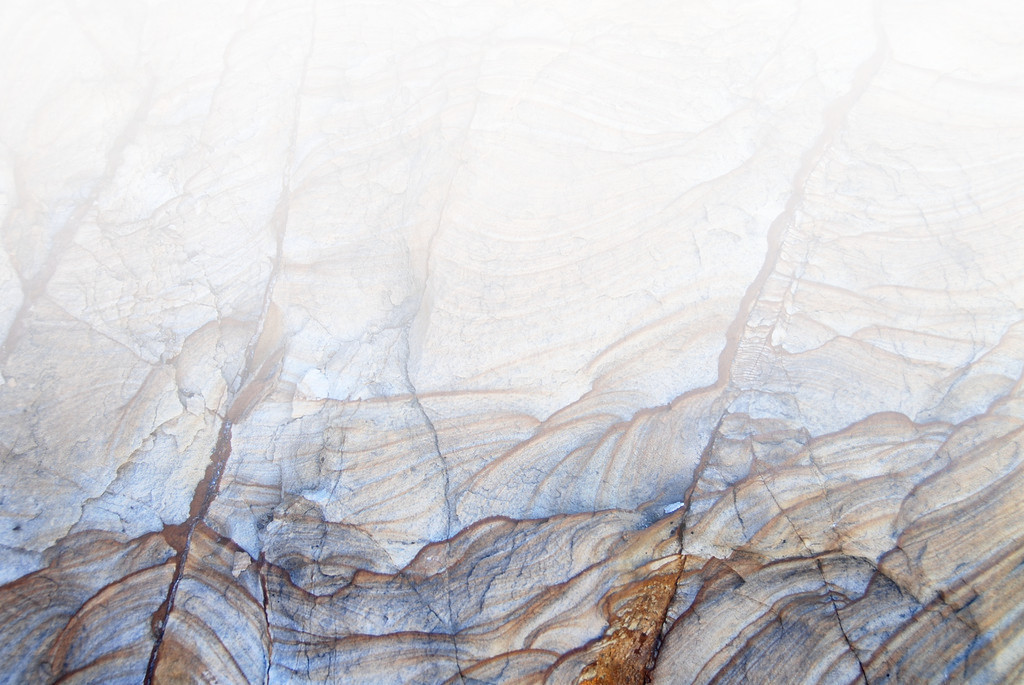
\includegraphics[width=1.02\textwidth]{graphics/nice_rock_colors_grad.jpg}\hfil
                }
            \vfil}
    }%
   
    
    \begin{frame}
        \centering
        \vspace{0.5cm}
        {\bf\large\inserttitle}\\
        \vspace{2mm}
        \textit{\insertauthor~ \textcolor{structure}{$\boldsymbol{|}$} \insertdate}
    \end{frame}
}

% \begin{frame}{Outline}
% \tableofcontents
% \end{frame}


\begin{frame}{cíl projektu Endorse}
 
 Pravděpodobnostní charakterizace bezpečnosti EDZ\\
 v okolí konkrétního úložného místa\\
 založená na matematických modelech vzniku EDZ.
 
\end{frame}

\begin{frame}{Endorse modely}
 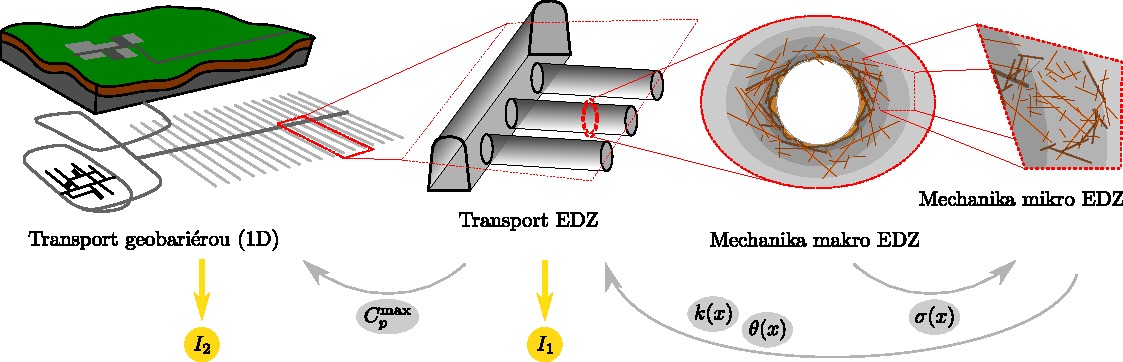
\includegraphics[width=\textwidth]{graphics/main_scheme.pdf}
\end{frame}


\begin{frame}{Transportní model}
Indikátory definovány pomocí transportního modelu podél díla.\\
Hotova první verze transportu.

\vspace{2ex}
{\bf Pevné vstupy}
\begin{itemize}
  \item geometrie (3 úložné vrty)
  \item max. tloušťka EDZ
  \item tok koncentrace na vnitřní hranici
  \item tlak na vnější hranici (z regionálního modelu)
\end{itemize}

\vspace{2ex}
{\bf Náhodné vstupy}
\begin{itemize}
 \item polohy makro puklin (rozměr nad 10m)
 \item porozita, permeabilita, difúzní parametry v masivu
\end{itemize}

\vspace{2ex}
{\bf Vlastnosti EDZ - z modelů mechaniky}\\
porozita, {\bf tenzor permeability}, difúzní parametry v masivu
\end{frame}


\begin{frame}{Makro model EDZ}

Pro modely predikce vodivosti a poruch:
\begin{itemize}
 \item 2D nebo 3D řez úložným vrtem + okolí
 \item nelineární mechanika s plasticitou/poškozením
 \item pole posunutí
 \item micro model pro permeabilitu a další vlastnosti EDZ
\end{itemize}

Základní varianta: parametry modelů fitovány z měření in-situ.
\end{frame}



\begin{frame}{Koncept predikce vlastností EDZ}
Víceškálová představa:
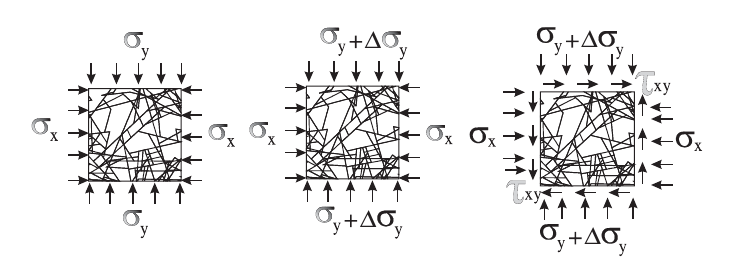
\includegraphics[width=\textwidth]{graphics/2D_fractures_loading.png}
\vspace{2ex}
Min, Jing: Numerical determination of the equivalent elastic compliance tensor
for fractured rock masses using the distinct element method, 2003
\end{frame}

\begin{frame}{Permeabilita}
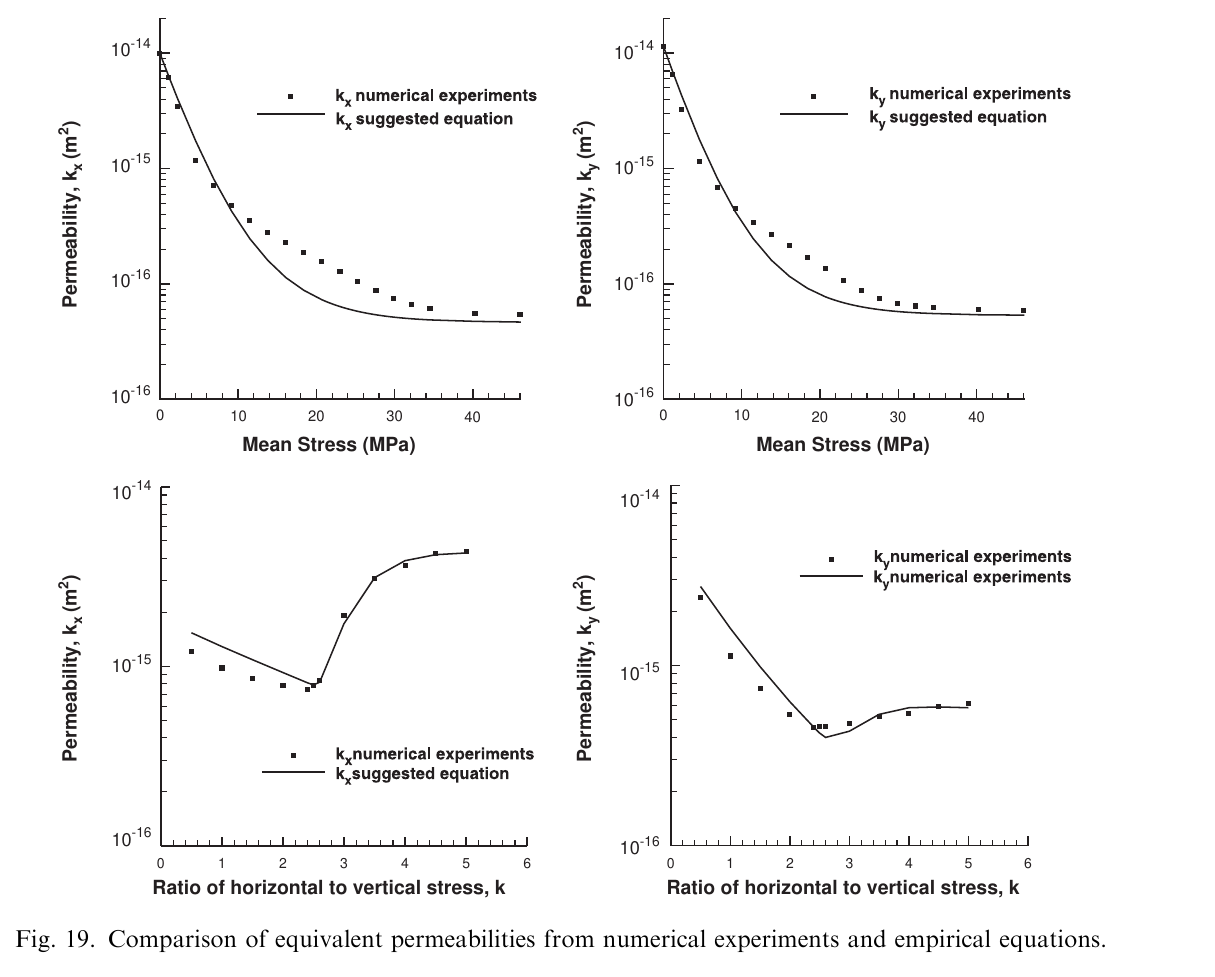
\includegraphics[width=\textwidth]{graphics/2D_equiv_permeabilty.png}
\vspace{2ex}
Min et al.: Stress-dependent permeability of fractured rock
masses: a numerical study, 2004
\end{frame}

% \begin{frame}{Microscale surogate}
% Fitování existujících emirických vztahů (Min, Rutquist) pomocí simulace zátěžových testů 
% mikroškálou. Možno aplikovat Bayesovu inverzi pro získání rozdělení parametrů těchto modelů.
% 
% \vspace{2ex}
% Fitování obecného polynomiálního surogate modelu.
% \end{frame}


\begin{frame}{Hotovo}
 \begin{itemize}
  \item definice indikátorů, modely transportu
  \item dílčí HM modely (něco s puklinami, něco s plasticitou) s puklinami
  \item generování náhodných puklin, 
  \item aplikace Bayesovské inverze na HM model
 \end{itemize}
 
 TODO:
 \begin{itemize}
  \item Dostatečně robustní simulátor pro mechaniku s plasticitou.
  \item Model pro experiment TSX. Aplikace Bayesovských metod na HM model s plasticitou.
  \item Model s kontakty na puklinách.
 \end{itemize}

\end{frame}

\begin{frame}{TSX}
 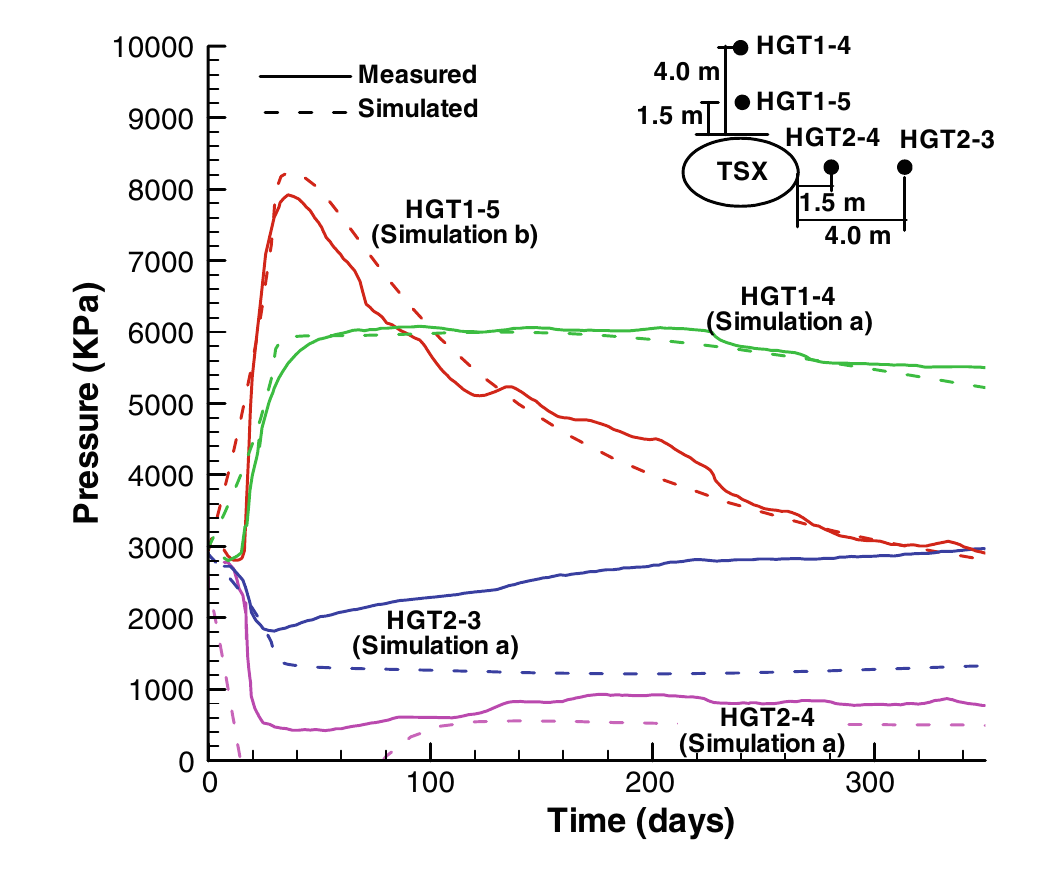
\includegraphics[width=0.9\textwidth]{graphics/TSX_measurement.png}
\end{frame}



\end{document}



